\documentclass{article}

% Language setting
% Replace `english' with e.g. `spanish' to change the document language
\usepackage[english]{babel}

% Set page size and margins
% Replace `letterpaper' \documentclass{article}
\usepackage{graphicx} % Required for inserting images
\usepackage{polski}
\usepackage[letterpaper,top=2cm,bottom=2cm,left=3cm,right=3cm,marginparwidth=1.75cm]{geometry}
\usepackage{amsmath}
\usepackage{graphicx}
\usepackage{algpseudocode}
\usepackage{array}
\usepackage{float}
\usepackage{pgfplots}
\pgfplotsset{compat=1.18}
\usepackage[colorlinks=true, allcolors=blue]{hyperref}

\title{Obliczenia naukowe lista 5}
\author{Stanisław Tomkowiak}
\date{4 stycznia 2024}

\begin{document}
\maketitle


\section*{Opis zadania}
Problem przedstawiony na liście 5 sprowadza się do rozwiązania układu równań liniowych:
\[
\texttt{Ax=b.}
\]
dla danej macierzy współczynników $\texttt{A} \in \mathbb{R}^{n \times n}$ i wektora prawych stron $\texttt{b} \in \mathbb{R}^n$, $n \geq 4$. Macierz \texttt{A} jest rzadką, tj. mającą dużą elementów zerowych, i blokową o następującej strukturze:
\[
    \texttt{A}=
    \begin{pmatrix}
        A_1    & C_1    & 0      & 0       & 0       & ...     & 0       \\
        B_2    & A_2    & C_2    & 0       & 0       & ...     & 0       \\
        0      & B_3    & A_3    & C_3     & 0       & ...     & 0       \\
        \vdots & \ddots & \ddots & \ddots  & \ddots  & \ddots  & \vdots  \\
        0      & ...    & 0      & B_{v-2} & A_{v-2} & C_{v-2} & 0       \\
        0      & ...    & 0      & 0       & B_{v-1} & A_{v-1} & C_{v-1} \\
        0      & ...    & 0      & 0       & 0       & B_v     & A_v     \\
    \end{pmatrix}
\]
$v=n/l$ zakładając, że $n$ jest podzielne przez $l$, gdzie $l \ge 2$ jest rozmiarem wszystkich kwadratowych
macierzy wewnętrznych (bloków):
$\texttt{A}_i \in \mathbb{R}^{l \times l}$, $\texttt{B}_i \in \mathbb{R}^{l \times l}$, $\texttt{C}_i \in \mathbb{R}^{l \times l}$, $i=1,...,v$. $\texttt{A}_i$ jest macierzą gęstą, $\texttt{B}_i, i \neq 1$ jest macierzą mającą elementy niezerowe tylko w dwóch ostatnich kolumnach, $\texttt{C}_i, i \neq v$ jest macierzą mającą elementy niezerowe tylko na przekątnej. Zakładamy, że $l=O(1)$. Dla bardzo dużych $n$ napotykamy problem dotyczący wymagań pamięciowych i czasowych. Zadanie polega na dostosowaniu użytych struktur oraz algorytmów do szczególnej postaci macierzy, aby z standardowego czasu $O(n^3)$ zredukować go do $O(n)$. Rozwiązanie układu równań liniowych:
\[
\texttt{Ax=b.}
\] mamy otrzymać i zbadać za pomocą czterech algorytmów:
\begin{itemize}
    \item Standardowego rozwiązania bez wyboru elementu głównego układu równań za pomocą eliminacji Gaussa.
    \item Standardowego rozwiązania z częściowym wyborem elementu głównego układu równań za pomocą eliminacji Gaussa.
    \item Rozwiązania bez wyboru elementu głównego układu równań z wyznaczonym rozkładem \texttt{LU}.
    \item Rozwiązania z częściowym wyborem elementu głównego układu równań z wyznaczonym rozkładem \texttt{LU}.

\section*{Rozwiązanie}
\subsection*{Struktura danych}
Klasyczny sposób przechowywania macierzy w postaci tablicy dwuwymiarowej jest tutaj nieskuteczny. Wynika to z tego, że w założeniach mamy, że n jest duże. W takim przypadku samo zapisanie tablicy zajmowałoby $O(n^2)$ miejsca. Z treści wiemy, że macierz jest rzadka co sprawia, że zapamiętalibyśmy bardzo dużo wartości równych $0$ co nie jest nam potrzebne. Musimy zatem znaleźć inną strukturę. Rozwiązaniem tego jest zapamiętywanie jedynie komórek niezerowych.

Język Julia udostępnia strukturę idealną do tego zadania. Znajduje się ona w pakiecie \texttt{SparseArrays}. Struktura nosi nazwę \texttt{SparseMatrixCSC}. Przechowuje ona trzy tablice. Pierwsza z numerami kolumn, druga z numerami wierszy i trzecia z wartościami. Czytając każdą z nich na tym samym indeksie dostaniemy numer wiersza, kolumny i wartość. Dzięki temu iterowanie po wierszach i kolumnach w żadnym stopniu nie uwzględnia iterowania po wartościach zerowych.
\subsection*{Eliminacja Gaussa}
\subsubsection*{Klasyczny algorytm i podstawy teoretyczne}
W sytuacji ogólnej dla gęstych macierzy układ równań ma postać:
\[ a_{11}^{(1)}x_1 + a_{12}^{(1)}x_2 + ... + a_{1n}^{(1)}x_n = b_1^{(1)} \]
\[ a_{21}^{(1)}x_1 + a_{22}^{(1)}x_2 + ... + a_{2n}^{(1)}x_n = b_2^{(1)} \]
\[ ... \]
\[ a_{n1}^{(1)}x_1 + a_{n2}^{(1)}x_2 + ... + a_{nn}^{(1)}x_n = b_n^{(1)} \]
W pierwszym kroku algorytmu eliminujemy zmienną $x_1$ z równań od 2-go do $n$-tego oraz mnożymy 1-sze równanie przez
\[ I_{i1} = \frac{a_{i1}^{(1)}}{a_{11}^{(1)}}, i = 2,...,n \]
i odejmujemy od pozostałych.
\par
Postępując dalej w ten sposób po 1-szym kroku układ wygląda w następujący sposób:
\[ a_{11}^{(1)}x_1 + a_{12}^{(1)}x_2 + ... + a_{1n}^{(1)}x_n = b_1^{(1)}  \]
\[ a_{22}^{(2)}x_2 + ... + a_{2n}^{(2)}x_n = b_2^{(2)} \]
\[ ... \]
\[ a_{n2}^{(2)}x_2 + ... + a_{nn}^{(2)}x_n = b_n^{(2)} \]
Po $k-1$ krokach otrzymujemy:
\[ a_{11}^{(1)}x_1 + a_{12}^{(1)}x_2 + ... + a_{1n}^{(1)}x_n = b_1^{(1)} \]
\[ a_{22}^{(2)}x_2 + ... + a_{2n}^{(2)}x_n = b_2^{(2)} \]
\[ ... \]
\[ a_{kk}^{(k)}x_k + ... + a_{kn}^{(k)}x_n = b_k^{(k)} \]
\[ ... \]
\[ a_{nk}^{(k)}x_{k} + ... + a_{nn}^{(k)}x_n = b_n^{(k)} \]
Eliminujemy zmienną $x_k$ z równań od $k+1$-szego do $n$-tego oraz mnożymy $k$-te równanie przez
\[ I_{ik} = \frac{a_{ik}^{(k)}}{a_{kk}^{(k)}}, i = k+1,...,n \]
i odejmujemy od pozostałych.
\par
Po $n-1$ krokach otrzymujemy układ z macierzą trójkątną górną:
\[ a_{11}^{(1)}x_1 + a_{12}^{(1)}x_2 + ... + a_{1n}^{(1)}x_n = b_1^{(1)} \]
\[ a_{22}^{(2)}x_2 + ... + a_{2n}^{(2)}x_n = b_2^{(2)} \]
\[ ... \]
\[ a_{nn}^{(n)}x_n = b_n^{(n)} \]
Na tej podstawie zakładając, że elementy na przekątnej są niezerowe, możemy wyznaczyć rozwiązanie układu równań w następujący sposób:
\[ x_n = \frac{b_n}{a_{nn}^{(n)}} \]
Dalej wyznaczamy $x_k$ dla $k=n-1,...,1$
\[ x_k = \frac{b_k^{(k)} - \sum_{j=k+1}^{n} a_{kj}^{(k)}x_j}{a_{kk}^{(k)}} \]
Taki algorytm ma złożoność obliczeniową $O(n^3)$ oraz złożoność pamieciową $O(n^2)$.
\subsubsection*{Wybór częściowy elementu głównego}
Algorytm w tej zależności wygląda bardzo podobnie. Jedyną zmiana polega na znalezieniu elementu takiego, że
\[ |a_{pk}^{(k)}| = \max_{k \leq i \leq n} |a_{ik}^{(k)}| \]
i przestawieniu w macierzy $A^{(k)}$ wiersza $p$-tego z $k$-tym oraz elementu $p$-tego z $k$-tym w wektorze prawych stron $b^{(k)}$. Dzięki temu zabiegowi zmniejszamy błąd względny.
\subsubsection*{Optymalizacja algorytmu}
Konkretna struktura macierzy \texttt{A} pozwoli  nam na znaczną optymalizację algorytmów. Mianowicie założeniem eliminacji Gaussa jest zerowanie elementów pod diagonalą. Większość tych elementów jeszcze przed użyciem algorytmu jest równa 0. Należy zatem zrewidować zakresy na których powinniśmy działać.

Zaczynając od kolumn maksymalnym wychyleniem pod diagonalę będzie rozmiar bloku $l$. Najbardziej wewnętrzna pętla powinna natomiast wykonywać się do czasu ostatniej nie zerowej wartości w wierszu. Sprawia to, że złożoność zmienia się z $O(n^3)$ na $O(n*l*l)$ a przy założeniu $O(l)=1$ daje nam złożoność na poziomie $O(n)$. 
\subsection*{Rozkład \texttt{LU}}

\subsubsection*{Klasyczny algorytm i podstawy teoretyczne}
Każdy krok pierwszego etapu eliminacji Gaussa można przestawić poprzez przemnożenie macierzy
\[ A^{(k+1)} = L^{(k)}A^{(k)}, b^{(k+1)} = L^{(k)}b^{(k)}, \]
gdzie
\[
    L^{(k)}=
    \begin{pmatrix}
        1 &        &            &   &  &        &   \\
          & \ddots &            &   &  &        &   \\
          &        & 1          &   &  &        &   \\
          &        & -I_{k+1,k} & 1 &  &        &   \\
          &        & -I_{k+2,k} &   &  &        &   \\
          &        & \vdots     &   &  & \ddots &   \\
          &        & -I_{k+n,k} &   &  &        & 1 \\
    \end{pmatrix}
\]
Zatem proces sprowadzenia macierzy $A^{(1)} = A$ do macierzy trójkątnej górnej $A^{(n)} = U$ można zapisać jako
\[ U = L^{(n-1)}...L^{(2)}L^{(1)}A \]
\[ A = (L^{(n-1)}...L^{(2)}L^{(1)})^{-1}U \]
\[ A = L^{(1)-1}L^{(2)-1}...L^{(n-1)-1}U \]
Oznaczamy $L = L^{(1)-1}L^{(2)-1}...L^{(n-1)-1}$.
\[
    L=
    \begin{pmatrix}
        1      &        &     &           &   \\
        I_{21} & 1      &     &           &   \\
        I_{31} & I_{32} & 1   &           &   \\
        \vdots & \vdots &     & \ddots    &   \\
        I_{n1} & I_{n2} & ... & I_{n,n-1} & 1 \\
    \end{pmatrix}
\]
W ten sposób pierwszy etap eliminacji Gaussa możemy równoważnie zapisać jako $A = LU$.

W realizacji algorytmu pamiętamy wszystko w jednej macierzy, gdzie elementy macieży $U$ są pamiętane jak wcześniej w górnym trójkącie i na przekątnej, a elementy macierzy $L$ w dolnym trójkącie, pamiętamy dodatkowo o tym, że ma ona jedynki na przekątnej, których nie trzeba zapisywać w pamięci.
\par
Rozkład LU wygląda zatem tak samo jak pierwszy etap eliminacji Gaussa, tylko zamiast zmieniać odpowiednie elementy w macierzy $b$, zapisujemy w dolnym trójkącie elementy macierzy $L$. Indeksy, po których się poruszamy pozostają takie same, czyli złożoność obliczeniowa i pamięciowa pozostaje $O(n)$.

Znając rozkład \texttt{A} = \texttt{LU} zadanie $\texttt{A}x = \texttt{b}$ sprowadzamy do
rozwiązania dwóch układów trójkątnych:
\par
\[
\texttt{L}y = \texttt{b}
\]
\[
\texttt{U}x = y
\]


\subsubsection*{Wybór częściowy elementu głównego}
Algorytm w tej zależności wygląda bardzo podobnie. Jedyną zmiana polega na znalezieniu elementu takiego, że
\[ |a_{pk}^{(k)}| = \max_{k \leq i \leq n} |a_{ik}^{(k)}| \]
i przestawieniu w macierzy $A^{(k)}$ wiersza $p$-tego z $k$-tym oraz zapisaniu w dodatkowej tablicy jakie wiersze zostały zamienione aby w kolejnym kroku odpowiednio zmodyfikować wektor \texttt{b}. Dzięki temu zabiegowi zmniejszamy błąd względny.
\subsubsection*{Optymalizacja algorytmu}
Podobnie jak w prypadku eliminacji Gaussa należy  zrewidować zakresy na których powinniśmy działać. Zakresy te są takie same. Sprawia to, że złożoność zmienia się z $O(n^3)$ na $O(n*l*l)$ a przy założeniu $O(l)=1$ daje nam złożoność na poziomie $O(n)$. 

\section*{Metodologia badania}
Aby łatwo porównać wyniki użyta została funkcja \texttt{blockmat} z modułu \texttt{matrixgen}. Za jej pomocą wygenerowane zostały macierze zgodne ze specyfikacją zadania o wielkości od $n=1000$ do $n=15000$ z krokiem równym $1000$. Pozostałe parametry to $l=4$ i wskaźnikiem uwarunkowania równym $ck=10$. Następnie dla wygenerowanych macierzy uruchomiono testy, które liczyły czas wykonania każdego algorytmu, zaalokowaną pamięć oraz błąd względny. Każdy test został wykonany 3 razy dla każdej funkcji aby wyeliminować błędy. Wektor \texttt{b} był wyliczany za pomocą funkcji \texttt{getB}.

\section*{Wyniki oraz interpretacja}
\subsection*{Eliminacja Gaussa bez częściowego wyboru elementu głównego}
\begin{figure}[H]
\centering
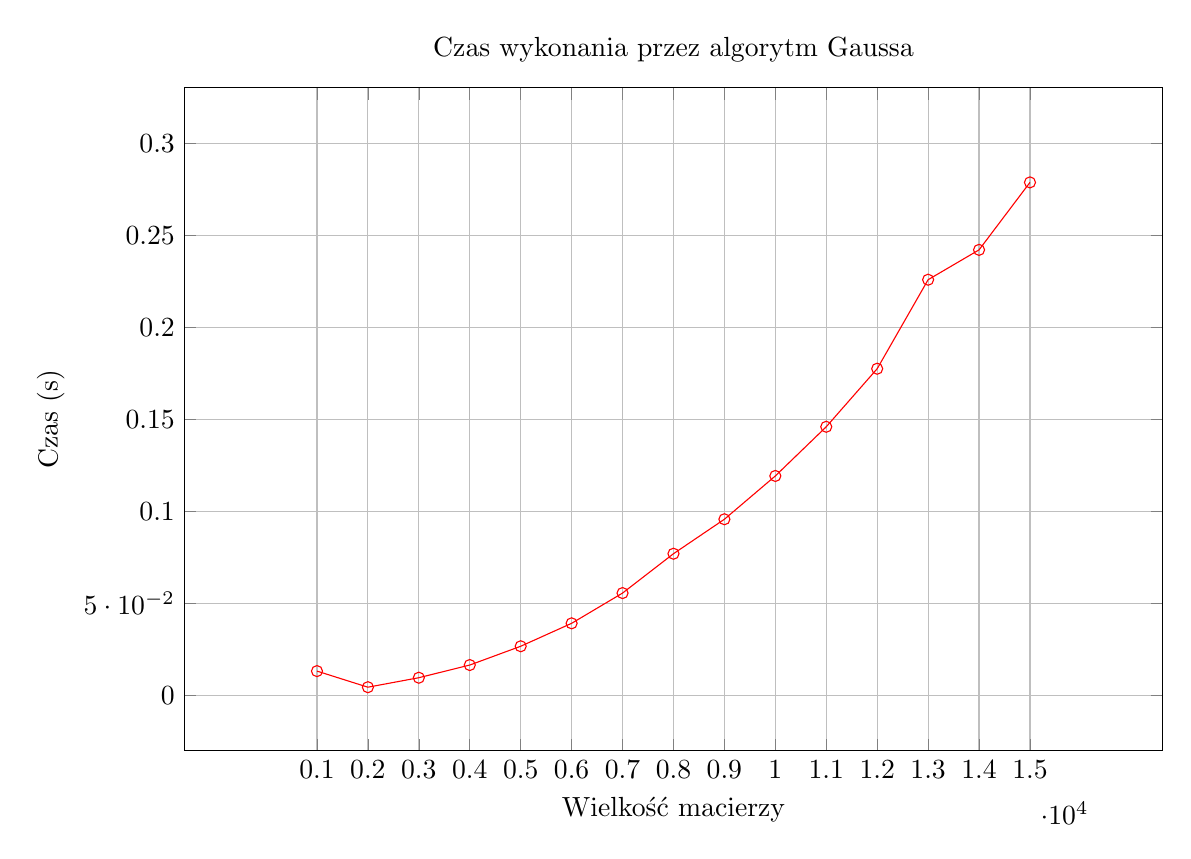
\begin{tikzpicture}
\begin{axis}[
    title={Czas wykonania przez algorytm Gaussa},
    xlabel={Wielkość macierzy},
    ylabel={Czas (s)},
    grid=major,
    width=14cm,
    height=10cm,
    enlargelimits=true,
    xmin=0, xmax=16000,
    ymin=0, ymax=0.3,
    xtick={1000, 2000, 3000, 4000, 5000, 6000, 7000, 8000, 9000, 10000, 11000, 12000, 13000, 14000, 15000},
    ytick={0, 0.05, 0.1, 0.15, 0.2, 0.25, 0.3},
    legend style={at={(0.5,-0.1)}, anchor=north, legend columns=2}
]
\addplot[
     color=red,
    mark=o,
    mark options={fill=red}
]
coordinates {
    (1000, 0.013251513666666666)
    (2000, 0.004508167333333333)
    (3000, 0.009661157333333333)
    (4000, 0.016543463999999997)
    (5000, 0.02673753666666667)
    (6000, 0.039199551)
    (7000, 0.055625651)
    (8000, 0.076999905)
    (9000, 0.09572264666666667)
    (10000, 0.11923486366666665)
    (11000, 0.14594576666666667)
    (12000, 0.17747684933333333)
    (13000, 0.22581286866666664)
    (14000, 0.242020239)
    (15000, 0.27866503633333334)
};
\end{axis}
\end{tikzpicture}
\end{figure}

Czas wykonania odbiega od założonego O(n) dzieje się tak ponieważ w rzeczywistości $O(l)\neq 1$. Czasy natomiast w porównaniu do niezoptymalizowanego algorytmu w dalszej mierze są bardzo dobre.
\begin{figure}[H]
\centering
\begin{tikzpicture}
\begin{axis}[
    title={Zużycie pamięci przez algorytm Gaussa},
    xlabel={Wielkość macierzy (n)},
    ylabel={Zużycie pamięci (KB)},
    grid=major,
    width=14cm,
    height=10cm,
    enlargelimits=true,
    xmin=0, xmax=16000,
    ymin=0, ymax=8000,
    xtick={1000, 2000, 3000, 4000, 5000, 6000, 7000, 8000, 9000, 10000, 11000, 12000, 13000, 14000, 15000},
    ytick={0, 1000, 2000, 3000, 4000, 5000, 6000, 7000},
    legend style={at={(0.5,-0.1)}, anchor=north, legend columns=2}
]
\addplot[
    color=red,
    mark=o,
    mark options={fill=red}
] 
coordinates {
    (1000, 486.78125)
    (2000, 488.953125)
    (3000, 1091.140625)
    (4000, 1130.203125)
    (5000, 1169.265625)
    (6000, 1208.328125)
    (7000, 3365.140625)
    (8000, 2431.953125)
    (9000, 2471.015625)
    (10000, 2510.078125)
    (11000, 2549.140625)
    (12000, 7018.578125)
    (13000, 7057.640625)
    (14000, 4978.953125)
    (15000, 5018.015625)
};
\end{axis}
\end{tikzpicture}
\end{figure}

\begin{figure}[H]
\centering
\begin{tikzpicture}
\begin{axis}[
    title={Błąd względny algorytmu Gaussa},
    xlabel={Wielkość macierzy (n)},
    ylabel={Błąd względny},
    grid=major,
    width=14cm,
    height=10cm,
    enlargelimits=true,
    xmin=0, xmax=16000,
    ymin=0, ymax=1e-13,
    xtick={1000, 2000, 3000, 4000, 5000, 6000, 7000, 8000, 9000, 10000, 11000, 12000, 13000, 14000, 15000},
    ytick={0, 1e-14, 2e-14, 3e-14, 4e-14, 5e-14, 6e-14, 7e-14, 8e-14},
    legend style={at={(0.5,-0.1)}, anchor=north, legend columns=2}
]
\addplot[
    color=red,
    mark=o,
    only marks, 
    mark options={fill=red}
] 
coordinates {
    (1000, 1.1609179125161992e-14)
    (2000, 1.2612284797402833e-14)
    (3000, 4.133321275316054e-14)
    (4000, 8.047440125690528e-15)
    (5000, 2.6484909348535394e-14)
    (6000, 4.2940550981274215e-14)
    (7000, 3.7566038367827404e-14)
    (8000, 5.4882335744644e-14)
    (9000, 8.109126735815906e-14)
    (10000, 3.970193093462694e-14)
    (11000, 1.9630106288058956e-14)
    (12000, 1.401914285187059e-14)
    (13000, 4.062541325787249e-14)
    (14000, 2.371000402378717e-14)
    (15000, 1.968754302149102e-14)
};
\end{axis}
\end{tikzpicture}
\end{figure}

Dla większości macierzy błąd względny był rzędu $10^{-14}$. Jest to akceptowalny wynik błędu. Można go jednak poprawić częściowym wyborem.

\subsection*{Eliminacja Gaussa z częściowym wyborem elementu głównego}
\begin{figure}[H]
\centering
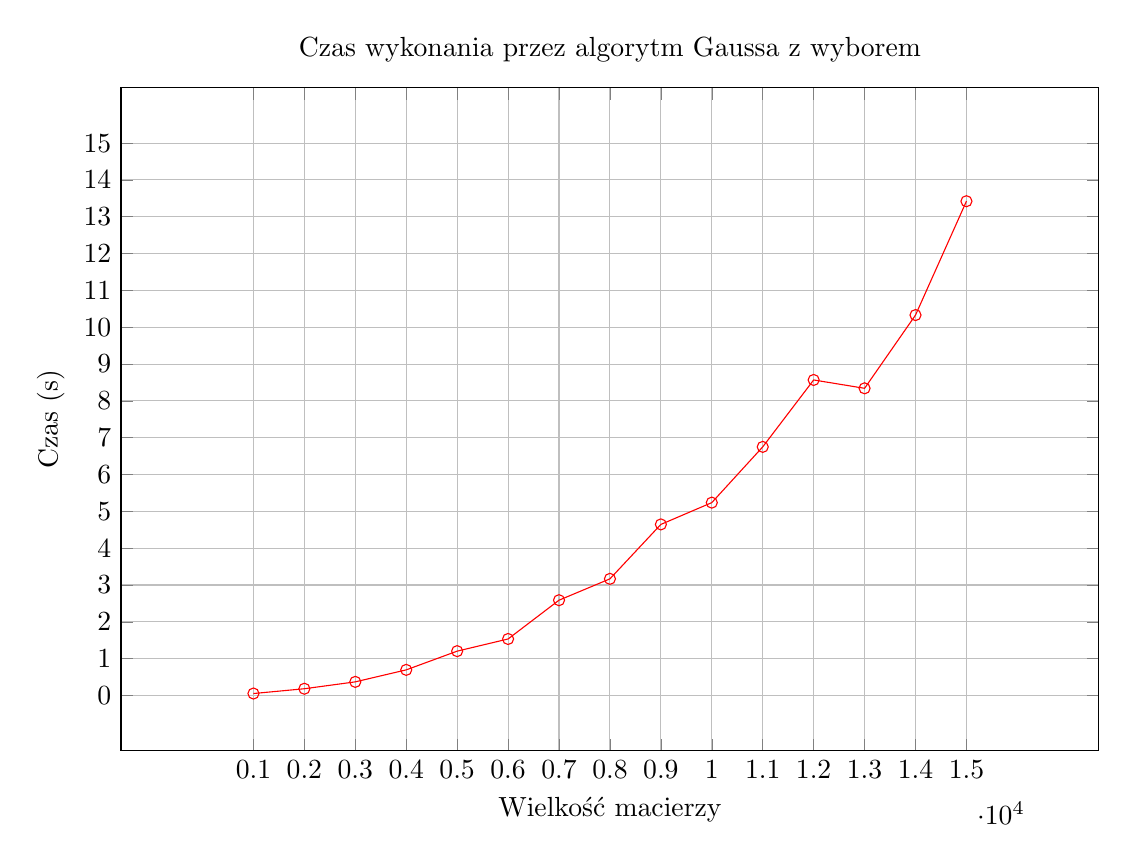
\begin{tikzpicture}
\begin{axis}[
    title={Czas wykonania przez algorytm Gaussa z wyborem},
    xlabel={Wielkość macierzy},
    ylabel={Czas (s)},
    grid=major,
    width=14cm,
    height=10cm,
    enlargelimits=true,
    xmin=0, xmax=16000,
    ymin=0, ymax=15,
    xtick={1000, 2000, 3000, 4000, 5000, 6000, 7000, 8000, 9000, 10000, 11000, 12000, 13000, 14000, 15000},
    ytick={0, 1, 2, 3, 4, 5, 6, 7, 8, 9, 10, 11, 12, 13, 14, 15},
    legend style={at={(0.5,-0.1)}, anchor=north, legend columns=2}
]
\addplot[
     color=red,
    mark=o,
    mark options={fill=red}
]
coordinates {
      (1000, 0.053559455666666665)
    (2000, 0.18358876999999998)
    (3000, 0.3703670606666667)
    (4000, 0.6960262086666665)
    (5000, 1.2044385523333334)
    (6000, 1.5350171556666667)
    (7000, 2.5880551026666665)
    (8000, 3.167809814)
    (9000, 4.6459639956666665)
    (10000, 5.237478698333334)
    (11000, 6.751425478333334)
    (12000, 8.568462896666666)
    (13000, 8.341668272666666)
    (14000, 10.330501243999999)
    (15000, 13.422293556)
};
\end{axis}
\end{tikzpicture}
\end{figure}
Czas wykonania odbiega od założonego O(n) dzieje się tak, ponieważ w rzeczywistości $O(l)\neq 1$. Czasy natomiast w porównaniu do niezoptymalizowanego algorytmu w dalszej mierze są bardzo dobre. Dodatkowo możemy zauważyć, że czasy są większe niż czasy eliminacji Gaussa bez wyboru. Zjawisko to zachodzi, ponieważ musimy dodatkowo odpowiednio permutować macierz oraz wektor \texttt{b}.
\begin{figure}[H]
\centering
\begin{tikzpicture}
\begin{axis}[
    title={Zużycie pamięci przez algorytm Gaussa},
    xlabel={Wielkość macierzy (n)},
    ylabel={Zużycie pamięci (KB)},
    grid=major,
    width=14cm,
    height=10cm,
    enlargelimits=true,
    xmin=0, xmax=16000,
    ymin=0, ymax=3.2e7,
    xtick={1000, 2000, 3000, 4000, 5000, 6000, 7000, 8000, 9000, 10000, 11000, 12000, 13000, 14000, 15000},
    ytick={0,0.5e7,  1e7, 1.5e7, 2e7, 2.5e7, 3e7},
    legend style={at={(0.5,-0.1)}, anchor=north, legend columns=2}
]
\addplot[
    color=red,
    mark=o,
    mark options={fill=red}
] 
coordinates {
    (1000, 137176.125)
    (2000, 545658.0)
    (3000, 1.20264534375e6)
    (4000, 2.1626680625e6)
    (5000, 3.370074875e6)
    (6000, 4.7649744375e6)
    (7000, 6.62775721875e6)
    (8000, 8.6928630625e6)
    (9000, 1.0886994375e7)
    (10000, 1.34171403125e7)
    (11000, 1.635931471875e7)
    (12000, 1.979875075e7)
    (13000, 2.29481823125e7)
    (14000, 2.659553878125e7)
    (15000, 3.04612905e7)
};
\end{axis}
\end{tikzpicture}
\end{figure}
Jest alokowane znacznie więcej pamięci niż w eliminacji bez wyboru. Znowu jest to kwestia permutowania macierzy.
\begin{figure}[H]
\centering
\begin{tikzpicture}
\begin{axis}[
    title={Błąd względny algorytmu Gaussa z wyborem},
    xlabel={Wielkość macierzy (n)},
    ylabel={Błąd względny},
    grid=major,
    width=14cm,
    height=10cm,
    enlargelimits=true,
    xmin=0, xmax=16000,
    ymin=0, ymax=1e-15,
    xtick={1000, 2000, 3000, 4000, 5000, 6000, 7000, 8000, 9000, 10000, 11000, 12000, 13000, 14000, 15000},
    ytick={0, 1e-16, 2e-16, 3e-16, 4e-16, 5e-16, 6e-16, 7e-146, 8e-16},
    legend style={at={(0.5,-0.1)}, anchor=north, legend columns=2}
]
\addplot[
    color=red,
    mark=o,
    only marks, 
    mark options={fill=red}
] 
coordinates {
    (1000, 4.617380053532766e-16)
    (2000, 4.777959296603251e-16)
    (3000, 4.628667009267583e-16)
    (4000, 4.581637676492595e-16)
    (5000, 4.463455571899844e-16)
    (6000, 4.2041894849163127e-16)
    (7000, 4.443785665843299e-16)
    (8000, 4.4368657147537686e-16)
    (9000, 4.518287937705369e-16)
    (10000, 4.368272626587955e-16)
    (11000, 4.47057964636014e-16)
    (12000, 4.457295417766688e-16)
    (13000, 4.476426521544921e-16)
    (14000, 4.443706415129202e-16)
    (15000, 4.534378815829483e-16)
};
\end{axis}
\end{tikzpicture}
\end{figure}

Błąd względny jednak jest dużo mniejszy niż w eliminacji bez wyboru. Wpływ na to ma wybieranie elementu głównego. Wyeliminowanie elementów bliskich zeru z przekątnej macierzy znacznie poprawiło błąd względny, który w każdym przypadku jest teraz rzędu epsilona maszynowego.
\subsection*{Rozkład LU bez wyboru elementu głównego}
\begin{figure}[H]
\centering
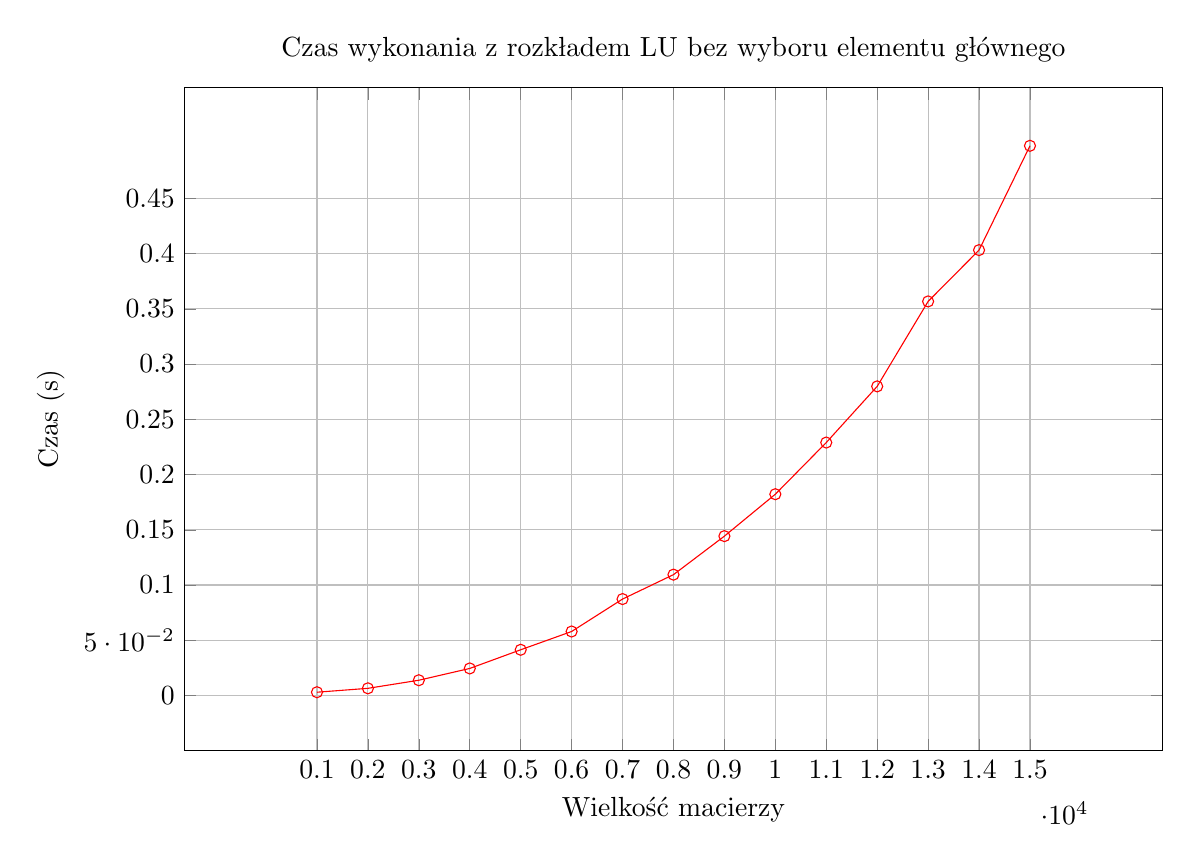
\begin{tikzpicture}
\begin{axis}[
    title={Czas wykonania z rozkładem LU bez wyboru elementu głównego},
    xlabel={Wielkość macierzy},
    ylabel={Czas (s)},
    grid=major,
    width=14cm,
    height=10cm,
    enlargelimits=true,
    xmin=0, xmax=16000,
    ymin=0, ymax=0.5,
    xtick={1000, 2000, 3000, 4000, 5000, 6000, 7000, 8000, 9000, 10000, 11000, 12000, 13000, 14000, 15000},
    ytick={0, 0.05, 0.1, 0.15, 0.2, 0.25, 0.3, 0.35, 0.4, 0.45},
    legend style={at={(0.5,-0.1)}, anchor=north, legend columns=2}
]
\addplot[
     color=red,
    mark=o,
    mark options={fill=red}
]
coordinates {
    (1000, 0.0029785093333333334)
    (2000, 0.006506326)
    (3000, 0.013830494666666667)
    (4000, 0.02450131633333334)
    (5000, 0.041396599)
    (6000, 0.05794532)
    (7000, 0.087296112)
    (8000, 0.10940000133333333)
    (9000, 0.14425730533333334)
    (10000, 0.18220815633333332)
    (11000, 0.22897325233333335)
    (12000, 0.27982033933333333)
    (13000, 0.356717624)
    (14000, 0.403156874)
    (15000, 0.49756790933333334)
};
\end{axis}
\end{tikzpicture}
\end{figure}
\begin{figure}[H]
\centering
\begin{tikzpicture}
\begin{axis}[
    title={Zużycie pamięci z rozkładem LU bez wyboru elementu głównego},
    xlabel={Wielkość macierzy (n)},
    ylabel={Zużycie pamięci (KB)},
    grid=major,
    width=14cm,
    height=10cm,
    enlargelimits=true,
    xmin=0, xmax=16000,
    ymin=0, ymax=8000,
    xtick={1000, 2000, 3000, 4000, 5000, 6000, 7000, 8000, 9000, 10000, 11000, 12000, 13000, 14000, 15000},
    ytick={0, 1000, 2000, 3000, 4000, 5000, 6000, 7000},
    legend style={at={(0.5,-0.1)}, anchor=north, legend columns=2}
]
\addplot[
    color=red,
    mark=o,
    mark options={fill=red}
] 
coordinates {
    (1000, 433.78125)
    (2000, 1429.46875)
    (3000, 1043.78125)
    (4000, 1067.21875)
    (5000, 1090.65625)
    (6000, 1114.09375)
    (7000, 3255.28125)
    (8000, 2306.46875)
    (9000, 2329.90625)
    (10000, 2353.34375)
    (11000, 2376.78125)
    (12000, 6830.59375)
    (13000, 6854.03125)
    (14000, 4759.71875)
    (15000, 4783.15625)
};
\end{axis}
\end{tikzpicture}
\end{figure}

\begin{figure}[H]
\centering
\begin{tikzpicture}
\begin{axis}[
    title={Błąd względny rozkładu LU bez wyboru elementu głównego},
    xlabel={Wielkość macierzy (n)},
    ylabel={Błąd względny},
    grid=major,
    width=14cm,
    height=10cm,
    enlargelimits=true,
    xmin=0, xmax=16000,
    ymin=0, ymax=1e-13,
    xtick={1000, 2000, 3000, 4000, 5000, 6000, 7000, 8000, 9000, 10000, 11000, 12000, 13000, 14000, 15000},
      ytick={0, 1e-14, 2e-14, 3e-14, 4e-14, 5e-14, 6e-14, 7e-14, 8e-14, 9e-14, 1e-13},
    legend style={at={(0.5,-0.1)}, anchor=north, legend columns=2}
]
\addplot[
    color=red,
    mark=o,
    only marks, 
    mark options={fill=red}
] 
coordinates {
    (1000, 1.1609179125161992e-14)
    (2000, 1.2612284797402833e-14)
    (3000, 4.133321275316054e-14)
    (4000, 8.047440125690528e-15)
    (5000, 2.6484909348535394e-14)
    (6000, 4.2940550981274215e-14)
    (7000, 3.7566038367827404e-14)
    (8000, 5.4882335744644e-14)
    (9000, 8.109126735815906e-14)
    (10000, 3.970193093462694e-14)
    (11000, 1.9630106288058956e-14)
    (12000, 1.401914285187059e-14)
    (13000, 4.062541325787249e-14)
    (14000, 2.371000402378717e-14)
    (15000, 1.968754302149102e-14)
};

\end{axis}
\end{tikzpicture}
\end{figure}
Wyniki zbliżone do otrzymanych w wyniku eliminacji Gaussa.
\subsection*{Rozkład LU z częściowym wyborem elementu głównego}
\begin{figure}[H]
\centering
\begin{tikzpicture}
\begin{axis}[
    title={Czas wykonania z rozkładem LU z częściowym wyborem elementu głównego},
    xlabel={Wielkość macierzy},
    ylabel={Czas (s)},
    grid=major,
    width=14cm,
    height=10cm,
    enlargelimits=true,
    xmin=0, xmax=16000,
    ymin=0, ymax=15,
    xtick={1000, 2000, 3000, 4000, 5000, 6000, 7000, 8000, 9000, 10000, 11000, 12000, 13000, 14000, 15000},
    ytick={0, 1, 2, 3, 4, 5, 6, 7, 8, 9, 10, 11, 12, 13, 14, 15},
    legend style={at={(0.5,-0.1)}, anchor=north, legend columns=2}
]
\addplot[
     color=red,
    mark=o,
    mark options={fill=red}
]
coordinates {
      (1000, 0.11808253666666667)
    (2000, 0.23158035633333332)
    (3000, 0.4093542620000001)
    (4000, 0.8701381759999999)
    (5000, 1.3107615536666666)
    (6000, 1.581473472)
    (7000, 2.614686267333333)
    (8000, 3.354114404666667)
    (9000, 4.160220422999999)
    (10000, 5.622563145333333)
    (11000, 5.714594944000001)
    (12000, 8.476989288)
    (13000, 9.428946902333331)
    (14000, 10.784709209333334)
    (15000, 12.426580608333333)
};
\end{axis}
\end{tikzpicture}
\end{figure}
\begin{figure}[H]
\centering
\begin{tikzpicture}
\begin{axis}[
    title={Zużycie pamięci z rozkładem LU z częściowym wyborem elementu głównego},
    xlabel={Wielkość macierzy (n)},
    ylabel={Zużycie pamięci (KB)},
    grid=major,
    width=14cm,
    height=10cm,
    enlargelimits=true,
    xmin=0, xmax=16000,
    ymin=0, ymax=2.2e7,
    xtick={1000, 2000, 3000, 4000, 5000, 6000, 7000, 8000, 9000, 10000, 11000, 12000, 13000, 14000, 15000},
    ytick={0,0.5e7,  1e7, 1.5e7, 2e7 },
    legend style={at={(0.5,-0.1)}, anchor=north, legend columns=2}
]
\addplot[
    color=red,
    mark=o,
    mark options={fill=red}
] 
coordinates {
    (1000, 446.078125)
    (2000, 137176.125)
    (3000, 433.78125)
    (4000, 141051.015625)
    (5000, 141051.015625)
    (6000, 559980.046875)
    (7000, 1.231285921875e6)
    (8000, 2.218904265625e6)
    (9000, 3.455398921875e6)
    (10000, 4.892225390625e6)
    (11000, 6.799048859375e6)
    (12000, 8.907748421875e6)
    (13000, 1.1166289921875e7)
    (14000, 1.3744214640625e7)
    (15000, 1.6756148328125e7)
};
\end{axis}
\end{tikzpicture}
\end{figure}

\begin{figure}[H]
\centering
\begin{tikzpicture}
\begin{axis}[
    title={Błąd względny rozkładu LU z częściowym wyborem elementu głównego},
    xlabel={Wielkość macierzy (n)},
    ylabel={Błąd względny},
    grid=major,
    width=14cm,
    height=10cm,
    enlargelimits=true,
    xmin=0, xmax=16000,
    ymin=0, ymax=1e-15,
    xtick={1000, 2000, 3000, 4000, 5000, 6000, 7000, 8000, 9000, 10000, 11000, 12000, 13000, 14000, 15000},
    ytick={0, 1e-16, 2e-16, 3e-16, 4e-16, 5e-16, 6e-16, 7e-146, 8e-16},
    legend style={at={(0.5,-0.1)}, anchor=north, legend columns=2}
]
\addplot[
    color=red,
    mark=o,
    only marks, 
    mark options={fill=red}
] 
coordinates {
    (1000, 4.617380053532766e-16)
    (2000, 4.777959296603251e-16)
    (3000, 4.628667009267583e-16)
    (4000, 4.581637676492595e-16)
    (5000, 4.463455571899844e-16)
    (6000, 4.2041894849163127e-16)
    (7000, 4.443785665843299e-16)
    (8000, 4.4368657147537686e-16)
    (9000, 4.518287937705369e-16)
    (10000, 4.368272626587955e-16)
    (11000, 4.47057964636014e-16)
    (12000, 4.457295417766688e-16)
    (13000, 4.476426521544921e-16)
    (14000, 4.443706415129202e-16)
    (15000, 4.534378815829483e-16)
};
\end{axis}
\end{tikzpicture}
\end{figure}
Wyniki zbliżone do otrzymanych w wyniku eliminacji Gaussa.
\section*{Wnioski}
Metoda rozwiązywania układu przy pomocy rozkładu LU cierpi na te same bolączki co eliminacja Gaussa. Wyniki są bardzo podobne. Zyskałaby ona jednak bardzo w momencie potrzeby wyliczenia rozwiązania dla różnych b. W takiej sytuacji liczylibyśmy tylko raz rozkład LU, co sprawiłoby, że wyniki byłyby miażdżące eliminację Gaussa. Obie metody: z częściowym wyborem oraz bez takiego wyboru są skuteczne. Wybór odpowiedniej powinien zależeć od tego, czy bardziej zależy nam na czasie, czy na jak najbardziej dokładnych wyliczeniach.
\end{document}